\chapter{Trusted computing}
Nowadays, the modern computing system is made up of many highly
distributed components.

Let's take into consideration the typical distributed infrastructure,
it's made up of a cloud for storage and computation, which communicate
with other devices outside its cluster, such as IoT devices, via edge
routers. Securing all those components it's a real challenge, because
each of those devices could be different, as well as their
communication technologies(Wired, Wireless, etc.). 

While in the past we had physical components, nowadays the trend is
\textbf{softwarization of the components} on top of a generic
commodity hardware, with "tools" such as SDN, NVF, etc.
\begin{boxH}
  As a consequence, systems \textbf{more flexible} but \textbf{more
  vulnerable}.
\end{boxH}
After all, the larger the software base, the higher the probability of
bugs, especially in the software, but hardware bugs are to be taken 
into consideration as well. All this without even considering the
issue of software updates

One of the main issues nowadays is \textbf{trustworthiness}, that being if
something behaves exactly as expected. However, there are several problems
related to trust in this context:

\begin{itemize}
    \item Trust in the cloud provider(s)
    \item Trust in the network/edge provider(s)
    \item Low or no access control for edge- and end-devices
    \item Low-cost IoT devices (which typically imply low security)
    \item Personal devices (often managed by users with limited 
          security knowledge)
\end{itemize}

If possible, it is recommended to protect the infrastructure by
avoiding or blocking all the possible attacks, which is a basically
impossible task. If protection is not feasible, one should do the next
best thing, that being monitoring the state of the system for early
detection and reaction to attacks. IDS can help to this end, but they
can be eluded by the attacker, so the best solution is to provide 
\textbf{integrity verification}, meaning that the system has not been
tampered with, both of the software component as well as their
configuration.

Integrity concerns can be categorized into hardware and 
software aspects:

\begin{itemize}
  \item \textbf{Hardware:}
    \begin{itemize}
      \item Am I communicating with the correct (intended) node?
      \item Does it host the expected (physical) components? For this
        reason, each contry is developing their own components
    \end{itemize}
  \item \textbf{Software:}
    \begin{itemize}
      \item Am I communicating with the correct (intended) 
        software component?
      \item Is it correctly configured?
      \item Is the baseline software the expected one?
    \end{itemize}
\end{itemize}

As we just explained, trust is a big issue in modern computing, and 
in order to answer all those questions, we need to consider some
solutions.
\section{Trusted Execution Environment (TEE)}
Systems are complex, and its difficult to trust every single
component, but we can create a small environment that we can trust.
But first, let's give again a definition of what trust is.
\begin{boxH}
  Something sor someone is \textbf{trusted} if one can \textbf{rely}
  upon to \textbf{not compromise your security}, without any
  guarantees.
\end{boxH}

Similarly, something is \textbf{trustworthy} if it \textbf{will not
compromise your security}, thinking about whether it is safe to use
something or not.

If something is trustworthy it is trusted, but not vice versa.

Trusted Execution Environment is what you may choose to rely upon to
execute sensitive tasks, which are called \textbf{Trusted
Applications} (TA), and which one hope to be trustworthy. 

TEE were originally developer for smartphones, which made them
necessary due to the high number of apps running on the same
environment, some of those with critical data(CC numbers, etc.), but
nowadays they are used in a variety of devices.

\begin{figure}[H]
  \centering
  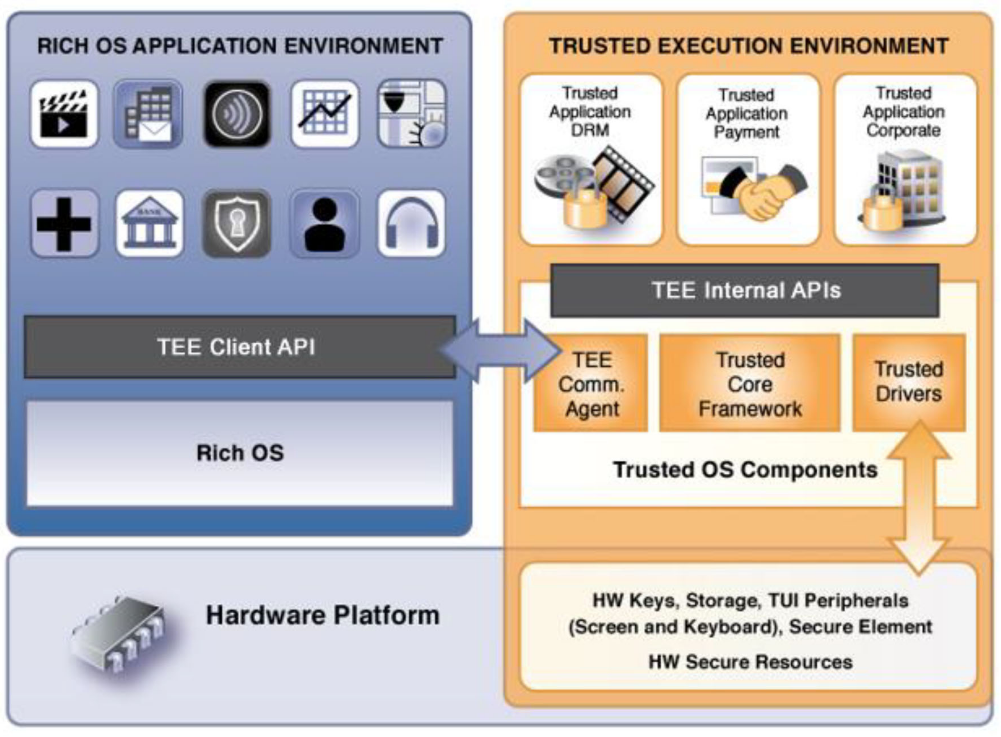
\includegraphics[width=0.5\textwidth]{img/Tee and REE.png}
  \label{fig:tee and ree}
  \caption{Trusted Execution Environment and Rich Execution
  Environment}
\end{figure}

As you can see from figure \ref{fig:tee and ree}, one one device can
run different enviroments at the same time On of those is a
\textbf{Rich Execution Environment} (REE), which is the normal
environment in which one runs any applications or OS. On the other
hand, the TEE is a separate environment isolated from the rest of the
system to run critical tasks and has access to some trusted ankles
like the hwardware keys, the secure storage, peripherals, etc.
TEE can only run on some specific hardware platform made up of trusted
components(not trustworthy, but trusted): the trusted drivers, the
core framework(the execution core) and a set of API accessible only
from trusted applications, the TEE communication agent 

In modern computing, TEE has become an important subject, especially
in the field of "confidential computing," which is actively promoted
by the Confidential Computing Consortium (CCC). The primary goal of
TEE is to protect "data in use," ensuring that nobody else can read or
write the data. Only authorized applications are allowed to process
the data. This approach contrasts with various cryptographic
techniques used to protect "data at rest" and "data in motion."

A key component of TEE, necessary to provide it's services, is the
\textbf{Root of Trust} (RoT), which is an element whose misbehavior
cannot be detected during runtime. The RoT must be \textbf{both
trusted and trustworthy}. It is also part of the Trusted Computing
Base (TCB), which is the set of hardware, firmware, and software
components critical to the system's security. Any vulnerability within
the TCB poses a significant threat to the system’s overall security.

\subsection{TEE Security Principles}

The security principles of a Trusted Execution Environment 
(TEE) involve the following:

\begin{itemize}
    \item Being part of the device's secure boot chain (based on a Root 
    of Trust) and verifying code integrity during each device boot.
    \item Hardware-based isolation from the device’s rich OS 
    environment to execute sensitive code.
    \item Isolation of Trusted Applications (TAs) from each other.
    \item Secure data storage, using a hardware-unique key accessible 
    only by the TEE OS to prevent unauthorized access, modification, 
    and any possibility of data exploitation on other devices.
    \item Privileged and secure access to peripherals (trusted path).
    \item Hardware isolation of peripherals (e.g., fingerprint sensors, 
    displays, touchpads) from the rich OS environment, controlled 
    only by the TEE during specific actions, with no visibility or 
    access by the Rich Execution Environment (REE), including 
    malware.
\end{itemize}

\section{Some TEE Implementations}
\subsection{Intel Identity Protection Technology (Intel IPT)}

Intel Identity Protection Technology (Intel IPT) is a security feature
that operates on a dual-CPU system within Intel processors. This
design leverages the Management Engine (ME), a dedicated CPU that
exists alongside the primary CPU in Intel processors. While the
primary CPU executes user tasks, the ME, integrated into the chipset,
can perform various management and security functions independently.
Typically, the ME is unused in consumer devices, but in corporate
environments, it can be activated even when the device is off via
features like wake-on-LAN, allowing remote management over Wi-Fi or
Ethernet.

Intel IPT uses the ME to run a \textbf{Java applet} isolated from the
main CPU, offering enhanced security for tasks such as cryptographic
key generation and storage, which integrates seamlessly with the
Windows Cryptographic API. Additionally, Intel IPT supports secure
One-Time Password (OTP) generation, as seen in applications like
VASCO's MYDIGIPASS.COM, which use the ME to securely store secrets for
OTPs. Another significant feature is secure PIN entry, where the
chipset manages video output to ensure the security of PIN input by
isolating it from the main system.

The ME's integration into the hardware, running on separate CPU
architecture, exemplifies a physically separated Trusted Execution
Environment (TEE), offering distinct security advantages by isolating
critical operations from the main processing tasks.

\subsection{ARM TrustZone}

ARM TrustZone is a Trusted Execution Environment (TEE) implemented in
certain ARM CPUs, designed to provide a secure and a normal mode
within the same processor. To achieve this, TrustZone extends the
CPU's bus with an additional "33rd bit" that signals whether the
processor is in secure or normal mode. This signal is exposed outside
the CPU, which enables secure peripherals and secure RAM by allowing
the system designer to control access to memory and devices based on
the security mode.

While the TrustZone framework is open and well-documented, it has some
limitations. TrustZone can only support a single secure enclave at a
time, and this security relies on software-based separation between
applications rather than on distinct hardware boundaries, making it
somewhat less secure than fully hardware-isolated environments. ARM is
actively working to expand TrustZone by introducing a third
operational mode to accommodate specific features like attestation.
However, adding this capability presents challenges due to backward
compatibility concerns, as ARM aims to preserve the success of its
platform without disrupting existing applications.

\subsection{Trustonic}

The main issue with TrustZone is that it only one secure enclave. 
To address this issue, Gemalto developed the Trusted Foundations 
system, and Giesecke+Devrient (G+D) created MobiCore. 
Both solutions effectively divide the single secure enclave into 
multiple enclaves by leveraging a smart-card operating system. 
Trustonic’s development is based on MobiCore, requiring 
license fees for implementing the code. Trustonic's TEE OS, 
named "Kinibi," includes enhancements such as version 500, 
which supports 64-bit Symmetric Multiprocessing (SMP) for 
embedded systems. Samsung Knox presents a similar approach 
but additionally incorporates secure boot functionality.

\subsection{Intel SGX}

Intel Software Guard Extensions (SGX) are tightly integrated with the
CPU, providing a hardware-based TEE by modifying memory management to
enhance security. SGX enables the creation of secure enclaves, which
are isolated execution environments protected from access by other
processes, even those with high priority. These enclaves achieve
memory isolation, ensuring that only the code within an enclave can
access its data, providing a high level of hardware-protected
separation.

When an SGX enclave is created, the Intel SGX architecture performs a
measurement, similar to Trusted Platform Module (TPM) practices, by
computing a hash of the executable loaded into the enclave. This
measurement-based security model is essential to SGX’s integrity,
ensuring that only approved code can run within an enclave.

For extended capabilities, SGX can be paired with Intel Identity
Protection Technology (IPT), allowing features such as a trusted
display. However, SGX itself is limited to CPU and memory protection
and does not provide secure input/output channels. When trusted
input-output is required, pairing with Intel IPT enables trusted
interaction with the display.

Intel initially made SGX-1 available across both consumer and
enterprise CPUs, but later revisions—specifically SGX-2—shifted focus
towards server-oriented environments. SGX-2 is now mainly available on
high-end CPUs, such as Intel’s Xeon series, used in data centers.
Furthermore, enclave creation within SGX requires special permissions
and the use of Intel-specific libraries, and all enclave-bound code
must be signed by Intel. This signing requirement means executable
code must be submitted to Intel to receive a signature, which may be a
barrier for some users.

\subsection{Keystone}

Keystone is an open-source framework designed for building Trusted
Execution Environments (TEEs). It allows developers to select only the
necessary features, which helps minimize the Trusted Computing Base
(TCB), because smaller the trust "surface" the better. The
architecture consists of an untrusted environment, such as a
general-purpose operating system, combined with multiple trusted and
segregated enclaves. Keystone is built on top of RISC-V, which offers
customizable open-source hardware options, including
Field-Programmable Gate Arrays (FPGAs) or System-on-Chip (SoC)
designs. The framework incorporates core components along with
cryptographic extensions and supports various execution modes,
including Machine(M), Supervisor(S), and User(U) modes. Additionally, it
features Physical Memory Protection (PMP), which has its
hardware-based access control to different pages of memory. That
avoids that one process can access the memory of another process,
either in general or specifically during a period of time. This helps
to safeguard memory and I/O operations, which are memory mapped.

Usually, TEEs are rigid and un-customizable, with many design
implementation dictated from the underlying hardware, for example
Intel SGX has a large software stack that is not customizable which
means a larger TCB, which is undesirable, AMD SEV
have the same issue and ARM TrustZone has a single TEE. 

The architecture is shown in figure \ref{fig:keystone}. Keystone is
structured to have a \textbf{Security Monition} as the only program
running in Machine mode(the highest privilege mode), which provides
which provides access control between any call coming from the upper
layers towards the hardware. It also provides an \textbf{untrusted
domain} where one can run any OS compatible with the RISC-V 
architecture(even Linux), which will run in Supervisor mode. 
Furthermore, to minimize the TCB, no hypervisor or base operating
systems are required.

On the other hand, one can have many \textbf{Enclaves}, which are 
isolated from the untrusted domain and from each other. Since they
dont need a general purpose OS, they run on a \textbf{Keystone 
Runtime}, which is a small OS that provides the necessary services 
to the specific application. On top of this, the \textbf{Keystone 
Application} runs, which is the actual application that the user 
wants to run.

\begin{figure}[H]
  \centering
  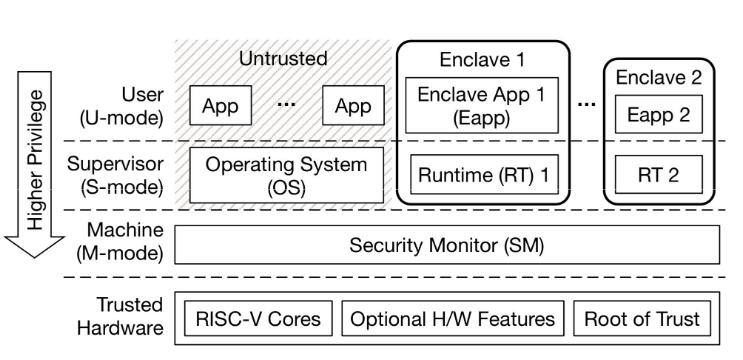
\includegraphics[width=0.6\textwidth]{img/keystone architecture.png}
  \label{fig:keystone}
  \caption{Keystone architecture}
\end{figure}

\begin{boxH}
  For the exam, read the bloody papers.
\end{boxH}

\section{Trusted computing and remote attestation}
Attacker would obviously like to inject malwares at the lowest level
possible, this is to remain undetected while still having access to
the largest part of the system. For this reason the ideal scenario is
to modify the OS is possible, or, alternatively boot an alternative
one under the control of the attacker by modifying the boot sequence
or even the bootloader.

It comes natural after this that the boot system and the OS should be
protected in order to trust the system: for boot sequencing we once
had the BIOS (Basic Input Output System), developed by specific
hardware vendors(no general purpose one available) which was very
difficult to protect, then we had UEFI (Unified Extensible Firmware
Interface) , which is more secure with native support for firmware
signature and verification. After this has been initialized, the OS
can be verified before activation.

So the manufacturer of the platform will sign the firmware, the UEFI,
and the hardware at boot will verify the signature. IF it fails, the
firmware has been tampered with, and the system will not boot. This
step is necessary to guarantee trust in the loaded OS.

\subsection{Rootkits}
This is the generic name for a tool that allows to have root access to
a machine. Of those, there are many kinds.

\paragraph{Firmware Rootkits} Firmware rootkits function by
overwriting the BIOS/UEFI or other hardware firmware. This allows the
rootkit to start running before the operating system even begins to
load.

\paragraph{Bootkits} Bootkits replace the bootloader of the operating
system, ensuring that the bootkit is loaded first when the node is
booted, which occurs before the OS itself initializes.

\paragraph{Kernel Rootkits} Kernel rootkits manipulate a section of
the OS kernel, enabling them to start automatically whenever the
operating system loads, embedding themselves within the core processes
of the OS.

\paragraph{Driver Rootkits} Driver rootkits disguise themselves as
trusted drivers used by the operating system (e.g., Windows) to
interact with hardware. By mimicking a legitimate driver, these
rootkits gain access to hardware resources while avoiding detection.
Don't confuse drivers rootkits with firmware ones, the firmware is
permanently stored in read-only memory, while drivers are part of the
OS and loaded at boot-time.

\section{Root of trust}
In general, protecting software with software can not always be the
best idea, as it may fail or have bugs. For this reason, we need
hardware support to protect the software.
At this end, we have a \textbf{Root of Trust}, which is a hardware 
component that is trusted to behave as expected, and is the foundation
for the chain of trust. The RoT should be always part of the Trusted
Computing Base because hardware is anyway operated by software or
firmware
\subsection{SW root-of-trust}

An example from HP Enterprise illustrates a method for firmware
self-protection, or software root-of-trust. HP Enterprise machines
implements a designated “signature” region at a small fixed location
within the final BIOS image, which is typically 16MB in size. Keep in
mind that this was developed before UEFI.

During manufacturing, the SHA-256 hash of the custom BIOS regions is
calculated. These regions include static code, BIOS version
information, and microcode, but not the hash itself, as its yet to be
initialized, at its only based on components that will never be
updated. The computed hash is then sent to an HPE signing server,
which returns a signed hash image (32 bytes) that includes the
signature and certificate information. This signed hash image is
stored in the BIOS “signature” region.

On power-up, the early BIOS code calculates a hash from the 
specified valid BIOS regions and verifies the validity of the 
stored “signature” contents. If the calculated hash matches 
the stored hash, the boot process proceeds; otherwise, the 
system halts, preventing further booting.

Of course, this method is not perfect, as it is still software-based 
and can be compromised. For example an attacker could replace the 
chip, which is soldered on the board, with a compromised one, or add
another memory chip on the free region of the board, which code will
be executed after the BIOS but before the OS without the integrity 
protection of the signature.

\subsection{HW root-of-trust}
The mechanism just described tries to verify firmware from the
firmware, but can we do better? Yes, we can use a hardware root of 
trust to verify the firmware. 

A hardware root-of-trust for firmware protection typically includes 
self-verification, where a static portion of the firmware authenticates 
the updatable section. This approach allows for an internal method 
of validating firmware integrity directly within the firmware itself. 
Alternatively, firmware verification can be managed by an external 
chip, offering a secure, independent means of affirming firmware 
authenticity.

For example take a look at figure \ref{fig:hw rot}, which shows a x86
Denverton CPU(which is quite old) and implements a 16MB SPI flash
memory, which stores the BIOS. It presents a multiplexer in front of
it that connects to both the CPU and an external cryptographic
microcontroller which can both use the SPI bus and drive the
multiplexer. So the decision of which chip can use the SPI bus is
taken by the external cryptographic microcontroller, which will verify
the integrity of the BIOS before allowing the CPU to boot.

Upon successful validation, this chip allows the x86 CPU to exit its
reset state; otherwise, the CPU remains in reset, ensuring security,
meaning that the chip is the true hardware root-of-trust.

The external chip may also include a fusing option, allowing a public
key hash, which is smaller than the public key, to be securely fused
and later used to verify the signature of the hash stored in the
BIOS's signature region. This validation process is similar to the
internal BIOS self-integrity check, with the added benefit of relying
on an external chip, making it the true hardware root-of-trust.

\begin{figure}[H]
  \centering
  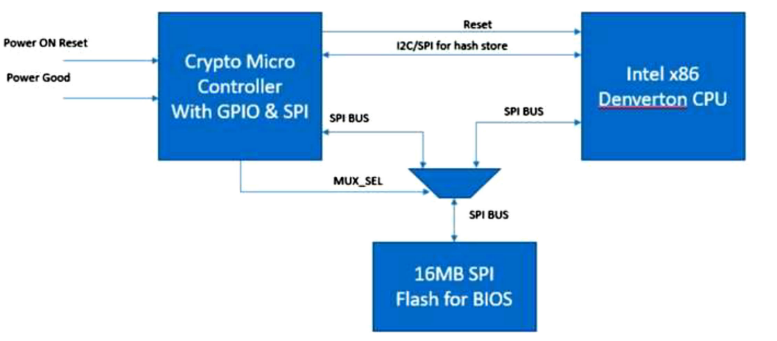
\includegraphics[width=0.6\textwidth]{img/Hw RoT verification.png}
  \label{fig:hw rot}
\end{figure}
\section{Boot Types}
Once we have been able to start the BIOS, the OS can be started.
Different types of boot processes provide varying levels of security
during system startup:

\paragraph{Plain Boot} A plain boot involves no security checks, 
leaving the platform vulnerable to unauthorized modifications.

\paragraph{Secure Boot} In a secure boot process, firmware verifies 
a signature before proceeding. If the verification fails, the platform 
halts, ensuring security from the earliest stages. This process is 
primarily hardware-based and verifies components up to the 
OS-loader.

\paragraph{Trusted Boot} A trusted boot involves the operating system
verifying signatures of critical OS components, such as drivers and
antimalware software. If any verification fails, system operations are
halted. You could have noticed that it assumes that the first part of
the boot up to the firmware was OK and performs verification only of
the operating system components. This type of boot is mainly
software-based and extends verification up to the operational state of
the OS.

\paragraph{Secure boot vs Trusted boot} With secure boot, if the
firmware(BIOS/UEFI/whatever) is compromised, it will not be loaded,
whereas with trusted boot, if the firmware is compromised, the OS
could still be loaded because the firmware is not verified. 


\paragraph{Measured Boot} During a measured boot, the system 
measures each component executed from boot through a defined 
point, denoted as \(X\). Unlike other boot types, measured boot 
does not halt operations if verification fails. Instead, it can securely 
report these measurements to an external verifier, providing 
ongoing insight into system integrity.

What has been just explained is shown in figure \ref{fig:boot types}.
Notice that the trusted drivers and the anti-malware are loaded before
the OS.
% 2 figures 
\begin{figure}[H]
  \centering
  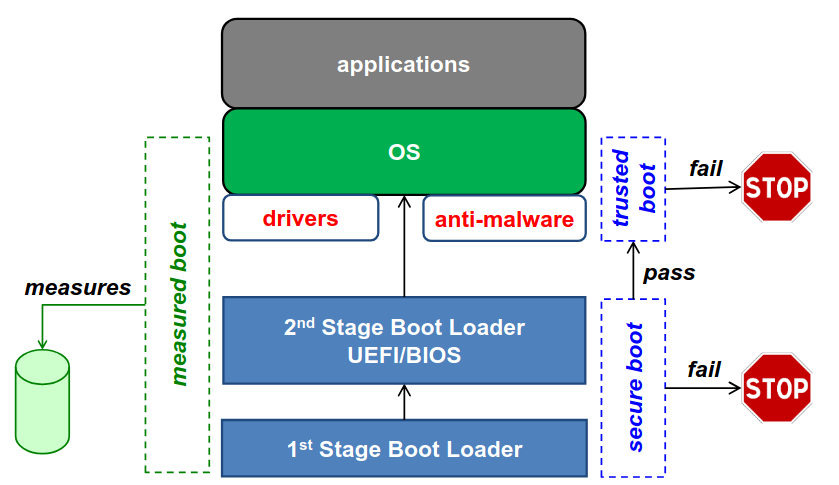
\includegraphics[width=0.6\textwidth]{img/boot types.png}
  \label{fig:boot types}
  \caption{Boot types}
\end{figure}

\subsection*{Windows Boot protection}

Windows 10 and Windows 11 implement a robust boot protection scheme
that combines Secure Boot, Trusted Boot, and Measured Boot to secure
the startup process against malicious interference, as shown in figure
\ref{fig:windows boot protection} . Secure Boot, which is managed by
the hardware manufacturer (e.g., Dell, Lenovo, HP), is the first line
of defense and prevents unauthorized firmware and bootloaders from
running. This step effectively blocks bootkits and ensures that only
trusted firmware initiates the boot sequence.

Following Secure Boot, Windows executes Trusted Boot, which verifies
and loads essential operating system components in a specific order:
first the OS loader, then the kernel, followed by system drivers,
critical system files, and Early Launch Anti-Malware (ELAM) drivers.
ELAM is a fundamental part of anti-malware solutions, as it starts
before any user-space process, offering early protection against
rootkits. The ELAM component must be submitted to Microsoft for
signature to ensure its integrity, enabling a secure foundation for
user-level anti-malware processes to operate later.

In conjunction with Secure Boot and Trusted Boot, Windows also
utilizes Measured Boot, which records each step in the boot process
for verification by an external verifier. If access is granted, this
verifier can query the system to confirm its boot integrity and detect
any potential tampering from the start. This integrated
approach—Secure Boot to lock down firmware, Trusted Boot to load and
verify core OS elements, and Measured Boot to maintain verifiable
logs—creates a strong defense against unauthorized modifications
during the boot process.


\begin{wrapfigure}{r}{0.5\textwidth}
  \centering
  \includegraphics[width=0.5\textwidth]{img/windows boot
  protection.png}
  \label{fig:windows boot protection}
\end{wrapfigure}

\section{Trusted Computing}

Trusted Computing encompasses systems and components designed 
to behave predictably and as expected. In this context, a component 
or platform is considered \textit{trusted} if it consistently performs 
according to predefined expectations, though this does not inherently 
mean it is secure or “good.” Trust in such systems requires verification 
against an expected behavior, rather than an implicit assumption of 
reliability.

A key concept within Trusted Computing is \textit{attestation}, which 
provides verifiable evidence of a platform’s state, allowing assessment 
against a known standard. Another fundamental concept is the 
\textit{Root of Trust}, an inherently trusted component within the 
system that forms the basis for verifying trustworthiness.

Trusted Computing schemes establish trust in a platform by 
identifying its hardware and software components, often through 
a \textit{Trusted Platform Module} (TPM). The TPM plays a crucial 
role in collecting and reporting component identities, offering a way 
to assess hardware and software configurations. This enables 
determination of whether a system’s behavior aligns with expected 
standards, thus supporting the establishment of trust in the platform’s 
integrity.

\subsection{Trusted Computing Base (TCB)}

\begin{boxH}
The Trusted Computing Base (TCB) refers to the \textbf{collection of
system resources}, including both hardware and software, that is
essential in upholding the security policy of a system. 
\end{boxH}

An essential aspect of the TCB is its resilience against compromise;
it must be able to protect itself from threats posed by any hardware
or software outside of the TCB itself.

It is important to note that the TPM \textbf{is not} synonymous with
the TCB of a system. Instead, the TPM serves as a tool for an
independent entity to assess whether the TCB has been compromised. 

In specific implementations, the TPM may also play a preventative
role, ensuring that the system does not start if the TCB fails to
initialize correctly, thus providing an additional layer of security
assurance.

\subsection{Root of Trust (RoT)}

\begin{boxH}
  The RoT refers to a component within a system that must reliably act
  in an expected manner, as any deviation in its behavior cannot be
  detected. 
\end{boxH}

The RoT is essential in establishing trust within a platform
and comprises several foundational components.

The \textbf{Root of Trust for Measurement} (RTM) is responsible for 
taking integrity measurements and transmitting these to the 
\textbf{Root of Trust for Storage} (RTS). Typically, the CPU executes 
the \textbf{Core Root of Trust for Measurement} (CRTM) at boot, 
serving as the first element of BIOS/UEFI code to initiate the 
chain of trust.

The RTS provides a shielded(no one can modify it) and secure storage
environment for critical integrity measurements.
The RTR securely reports the content stored in the RTS, thus enabling
verification of the system's integrity.

\subsection{Chain of Trust}

Our aim is, starting from the lowest level of the firmware, create a
\textbf{chain of trust}.

In a Chain of Trust, each component verifies the integrity of the next
component in sequence. Component A measures Component B and stores
this measurement in the RTS. Then, Component B measures Component C
and similarly stores the measurement in the RTS, continuing this
process down the chain.

Typically, Component A is the CRTM, which is part of the TCB. By using
the \textbf{Root of Trust for Reporting} (RTR), a verifier can
securely retrieve the measurements of Components B and C from the RTS.
For Components B and C to be trusted, Component A must itself be
trustworthy.

\subsection{Trusted Platform Module Overview}

The Trusted Platform Module is an inexpensive component, typically
costing less than 1 dollar, and is available on most servers, laptops,
and PCs. It is designed to be \textbf{tamper-resistant}, although it
is important to note that it is not entirely tamper-proof, meaning
that it is difficult to compromise it, but not impossible.

While the TPM provides security features, it is not a high-speed
cryptographic engine; in fact, it is relatively slow in terms of
processing speed, m.t. doing RSA signatures with it will take forever.
The TPM have to be certified with a \textbf{Common Criteria Evaluation
Assurance Level}(EAL) of 4 or higher, which indicates a certain level
of security assurance, which is quite good indeed.

As a passive component, the TPM requires the CPU to drive its
operations. It does not have the capability to prevent the boot
process; however, it can protect sensitive data and securely report
this information. Consequently, the TPM functions as both the RTS and
the RTR, but it does not serve as the RTM, because we'll perform the
measure and we'll store the results inside the TPM.

The TPM provides secure storage capabilities, functioning as a secure
storage component (RTS) with an extend-only approach. It can report
the content of this secure storage using a digital signature, thus
acting as a reporting entity (RTR). This means that every time that
memory is read outside the TMP, a digital signature computed with a
asymmetric key pair stored inside the TPM is attached to the data.

One of the critical features of the TPM is its hardware random number
generator, which supports various cryptographic algorithms, including
hashing, Message Authentication Code (MAC), and both symmetric and
asymmetric encryption. However, it is important to clarify that the
TPM is not a crypto accelerator, as its performance is relatively
slow.

The TPM also facilitates the secure generation of cryptographic keys
for limited use cases. It supports \textbf{binding}, which encrypts
data using the TPM bind key—a unique RSA key derived from a storage
key. What does that mean? Binding means that if you want to decrypt
this data, you can do that only on the platform that contains that
TPM. Because if you move the data to another platform, they are
encrypted with the key which is not there. This also means that if the
platform broke down, you can't decrypt the data anymore.

Additionally, the TPM allows for \textbf{sealing}, a process
similar to binding, but it also specifies the TPM state required for
the data to be decrypted, or unsealed. This means that the data can be 
decrypted only if the TPM is in a specific state, which is useful to
avoid tampering.

Furthermore, computer programs can utilize a TPM to authenticate
hardware devices. Each TPM chip is manufactured with a unique and
secret \textbf{Endorsement Key} (EK) that is burned in during
production, ensuring that the authenticity of the hardware can be
verified.

\subsection{TPM 1.2}

TPM 1.2 features a fixed set of cryptographic algorithms, which
include SHA-1, RSA, and optionally AES. This version of the TPM
provides a single storage hierarchy specifically for the platform
user, ensuring that key management and storage are centralized.

At the core of TPM 1.2 is a single root key known as the Storage Root
Key (SRK), which is typically an RSA-2048 key. This root key serves as
the foundation for other keys within the TPM, facilitating secure
storage and cryptographic operations.

Additionally, TPM 1.2 incorporates a built-in Endorsement Key (EK)
(RSA-2048) that provides a hardware identity for the platform. This EK
is essential for establishing the authenticity of the TPM and the
device it resides in. 

Another important thing of TPM 1.2 is its capability for sealing
only against the PCRs value, where the measurements are collected. 
\subsection{TPM 1.2}

TPM 1.2 features a fixed set of cryptographic algorithms, which
include SHA-1, RSA, and optionally AES. This version of the TPM
provides a single storage hierarchy specifically for the platform
user, ensuring that key management and storage are centralized.

At the core of TPM 1.2 is a single root key known as the Storage Root
Key (SRK), which is typically an RSA-2048 key. This root key serves as
the foundation for other keys within the TPM, facilitating secure
storage and cryptographic operations.

Additionally, TPM 1.2 incorporates a built-in Endorsement Key (EK)
that provides a hardware identity for the platform. This EK is
essential for establishing the authenticity of the TPM and the device
it resides in. 

Another important feature of TPM 1.2 is its capability for sealing
data to a Platform Configuration Register (PCR) value. This sealing
process ensures that the data can only be decrypted when the platform
is in a specific, verified state, enhancing the security of sensitive
information.
\begin{wrapfigure}{r}{0.5\textwidth}
  \centering
  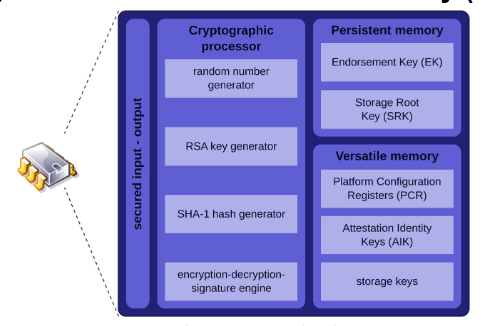
\includegraphics[width=0.5\textwidth]{img/TMP 1-2.png}
  \label{fig:tpm 1.2}
\end{wrapfigure}

\subsection{TPM 2.0}

TPM 2.0 introduces advanced cryptographic flexibility and supports a
range of algorithms, including SHA-1 for backward compatibility,
SHA-256, RSA, ECC-256, HMAC, and AES-128, providing robust options for
secure operations. This version organizes keys into three main
hierarchies: platform, storage, and endorsement. Each hierarchy can
support multiple keys and algorithms, enhancing security management
and allowing for versatile key applications based on specific needs.

A significant feature of TPM 2.0 is policy-based authorization,
enabling more sophisticated and adaptable access controls (in previous
version just one password was required). This policy
framework allows security measures to be tailored according to diverse
requirements and provides a structured way to enforce access
restrictions.

Additionally, TPM 2.0 includes platform-specific specifications
tailored to various application areas, including PC clients, mobile
devices, and automotive environments. Each of these specifications
addresses the unique security requirements of its respective platform,
ensuring that TPM 2.0 can meet the needs of a broad range of use
cases. However, most of the hardware manufacturers implements their
TPMs directly in the CPU or the chipset, meaning that one should check
when buying new hardware: in some cases the TPM is software based on
even virtualized on a dedicated VM thanks to the hypervisor.


\subsubsection{Implementations of TPM 2.0}

TPM 2.0 has several implementation forms, each designed to fit
different hardware and software architectures. The Discrete TPM is a
dedicated chip that implements TPM functionality within its own
tamper-resistant semiconductor package, providing robust security.

In contrast, the Integrated TPM is part of another chip and is not
required to implement tamper resistance. For example, Intel has
integrated TPMs in some of its chipsets, balancing functionality with
space and cost considerations.

The Firmware TPM is a software-only solution that operates within a
CPU's trusted execution environment. Major manufacturers such as AMD,
Intel, and Qualcomm have implemented firmware TPMs, allowing for
flexibility in system design.

Another form is the Hypervisor TPM, which offers a virtual TPM managed
by a hypervisor. This runs in an isolated execution environment and is
comparable to a firmware TPM in terms of security and functionality.

Finally, the Software TPM serves as a software emulator of a TPM,
primarily useful for development purposes. This allows developers to
test and implement TPM functionalities without needing dedicated
hardware.

\subsubsection{TPM 2.0 Three Hierarchies}

TPM 2.0 defines \textbf{three key hierarchies}, each serving distinct
purposes and managing different aspects of security and key storage.

The first hierarchy is the \textbf{Platform Hierarchy}, which is
dedicated to managing the platform’s firmware. This hierarchy utilizes
non-volatile (NV) storage for keys and data, ensuring that critical
firmware-related information is securely maintained.

The second is the \textbf{Endorsement Hierarchy}, which primarily
caters to the privacy administrator. But why we need a privacy admin?
In the early days of the TPM and the Trusted Computing Group (TCG),
there was concern over privacy implications. One issue was that every
time a device’s TPM measured and reported its state, it signed those
measurements with its unique RSA private key. This approach ensured
that the measurements were authentic and uniquely tied to the device,
which was valuable for verifying the integrity of the platform.
However, this method also had a drawback: it revealed the device’s
identity.
If each attestation came from a unique RSA key, it could be traced
back to the same machine each time, compromising privacy.
For this reasons we use different keys for different purposes(key of
the manufacturer, key to identify the owner, \ldots).

Similar to the Platform
Hierarchy, this one also provides storage for keys and data,
emphasizing the importance of privacy in the overall security
architecture.

Lastly, the \textbf{Storage Hierarchy} is designed for the platform’s
owner, who typically also acts as the privacy administrator. This
hierarchy features NV storage for keys and data, allowing for
efficient management of cryptographic assets.

Each of these hierarchies comes with dedicated authorization
mechanisms, such as passwords, and specific policies to govern access
and usage. Additionally, each hierarchy utilizes a unique seed for
generating the primary keys, further enhancing the security and
integrity of the TPM's operations.

\subsection{Using a TPM for Securely Storing Data}

Utilizing a TPM for securely storing data
involves several key considerations to ensure both security and
accessibility.

One primary advantage of using a TPM is its physical isolation. The
storage occurs within the TPM itself, specifically in NVRAM, which
helps safeguard sensitive information. This storage is very small, so
ut usually stores primary keys and permanent keys

To enhance security, Mandatory Access Control (MAC) mechanisms are
employed, which govern how data and keys are accessed within the TPM.
This cryptographic isolation ensures that even if data is stored
outside the TPM, such as on a platform's hard drive, it remains
protected.

When storing keys or data outside the TPM, it is crucial that the
information is encapsulated in a secure format, often referred to as a
blob. This blob must be protected, typically by encrypting it with a
key controlled by the TPM. The use of MAC further reinforces the
security measures, ensuring that access to the stored data is tightly
regulated.

\subsection{TPM Objects}

TPMs utilize various objects to manage cryptographic keys and secure
data. One of the primary types of objects within a TPM is the
\textbf{primary keys}, which includes endorsement keys and storage
keys. These keys are derived from one of the primary seeds stored
within the TPM. Notably, the TPM does not return the private value of
these keys; instead, they can be re-created using the same parameters,
assuming that the primary seed remains unchanged.

In addition to primary keys, TPMs also handle keys and sealed data
objects (SDOs). These objects are protected by a Storage Parent Key
(SPK), which is necessary within the TPM to load or create a key or
SDO. The randomness required for key generation and other
cryptographic functions is provided by the TPM's built-in Random
Number Generator (RNG). 

When a key is generated, the TPM returns the private part, which is
protected by the SPK. However, it is essential to note that this
private part must be stored securely, as its integrity is critical to
maintaining the overall security provided by the TPM.

\subsection{TPM Object Areas}

Trusted Platform Modules (TPMs) categorize the storage structure of
objects into distinct areas, each serving a specific purpose:

\begin{itemize}
  \item \textbf{Public Area:} This area is utilized to uniquely
    identify an object, providing essential information for the
    management of keys and data.

  \item \textbf{Private Area:} Containing the object's secrets, this
    area exists solely within the TPM. It is crucial for maintaining
    the confidentiality and integrity of the keys and data stored
    within the module.

  \item \textbf{Sensitive Area:} This consists of the encrypted
    private area, specifically designed for use when storing sensitive
    data outside of the TPM. It ensures that even when data is not
    housed within the TPM, it remains secure through encryption.
\end{itemize}

\subsection{TPM Platform Configuration Register (PCR)}

The Platform Configuration Register (PCR) serves as the TPM
implementation of Root of Trust for Storage (RTS) and is a core
mechanism for recording platform integrity. PCRs maintain their values
and can only be reset during a platform reset or through a hardware
signal, which ensures that any malicious code cannot manipulate or
retract its measurements.

PCRs are extended using a cumulative hash, following the formula:

\[
\text{PCR}_{\text{new}} = \text{hash}(\text{PCR}_{\text{old}} \, || \, \text{digest\_of\_new\_data})
\]
Basically, the new PCR value is the hash of the old PCR value and the 
new data. This process is repeated for each new piece of data that
needs to be added to the PCR.

This process is commonly referred to as the EXTEND operation (keep in
mind that it's not commutative).
Additionally, PCRs can be utilized to gate access to other TPM
objects. For example, BitLocker uses PCR values to seal disk
encryption keys, ensuring that the keys can only be accessed when the
platform is in a known and trusted state.

\subsection{Measured Boot}

Measured boot builds on secure and trusted boot principles by using
TPM functionality to verify system integrity throughout the boot
process. The key here is that a TPM is available—whether as a separate
chip or firmware module—enabling attestation at each step.

The process begins with the Core Root of Trust for Measurement (CRTM)
located in the boot ROM’s first-stage bootloader. This trusted
component takes the first measurement by capturing the state of the
next component in line, the second-stage bootloader, and stores this
in the TPM’s Platform Configuration Registers (PCRs). This baseline
measurement is critical, as it establishes initial trustworthiness for
everything that comes afterward.

Once the second-stage bootloader is loaded, it continues the process
by measuring the operating system, which can also measure subsequent
applications if needed. The idea is simple: measure each part of the
boot sequence and store these measurements in the PCRs, creating a
chain of trust from the very start.

The accumulated values in the PCRs provide a snapshot of the system’s
integrity, which an external verifier can check to confirm everything
is as expected. Though an internal verifier is possible, an external
one is often more reliable in case an attacker has compromised the
internal components. This setup allows measured boot to act as a
strong line of defense, verifying each stage and ensuring a trusted
environment.

\begin{figure}[H]
  \centering
  \includegraphics[width=0.6\textwidth]{img/Measured boot.png}
  \caption{Measured boot}
\end{figure}
\subsection{Remote attestation procedure}

Remote attestation leverages the values stored in the TPM’s PCRs
during the measured boot process, enabling an external verifier to
confirm the system's integrity. Here’s how it works:

First, an external verifier, which could be a trusted system on the
network, sends a unique challenge (often a nonce) to the device
holding the TPM. This challenge prevents replay attacks by ensuring
that each attestation session is fresh and unpredictable. The platform
then gathers the values of the PCRs requested by the verifier and
packages them along with the challenge.

This package of data—containing the PCR values and the response to the
nonce—is signed using a key unique to the device. This signed response
assures the verifier that it’s seeing legitimate measurements tied to
that specific device.

When the verifier receives the signed package, it performs several
checks:
\begin{enumerate}
  \item \textbf{Signature Validation}: It verifies the signature to
    ensure the data hasn’t been tampered with and is genuinely from the
    device.
  \item \textbf{Identity Validation}: It checks that the device’s
    identity matches expected values, using a stored list of authorized
    machines to confirm that the device is part of the network.
  \item \textbf{Measurement Validation}: Finally, the verifier compares
    the PCR values against known "golden values" stored in a database.
    These golden values reflect the expected configurations for each
    device type—taking into account variations in hardware, firmware,
    and software.
\end{enumerate}

If the PCR values match the golden values, the verifier can
confidently conclude that the system is in a known and trusted state.
If there’s a mismatch, an alert is raised, signaling that the device
may have been compromised or misconfigured.

This remote attestation process provides a robust way to ensure system
integrity across a network by verifying both the software status and
identity of each device, making it a valuable tool for network
security.

\begin{figure}[H]
  \centering
  \includegraphics[width=0.6\textwidth]{img/remote attestation
  procedure.png}
  \caption{Remote attestation procedure}
\end{figure}

\subsection{Management of Remote Attestation}

Remote attestation has been performed, and it has failed. What now?
Management of remote attestation is most important when the
attestation process fails. 

One critical aspect is whether to implement only boot attestation,
which is static, or to include periodic (dynamic) attestation as well.
This decision should take into account the attack model, especially
with respect to runtime vulnerabilities that could be exploited.

The \textbf{periodicity of the attestation} operation is another
important consideration, as it must align with the speed of potential
attacks. A cycle of operations which include the time
required for signature verification, protocol execution, and database
lookups, are typically in the range of several seconds due to the
inherent slowness of TPMs, and for some cases is acceptable, but for
others a window of exposure of even 5 seconds is excessive. 
And that is a limit, not of the attestation, but of the physical
implementation.

Another challenge in remote attestation management is
\textbf{whitelist generation}. This process can be complex in general
but may be less difficult in limited environments, such as Internet of
Things (IoT) devices, edge devices, Software-Defined Networking (SDN),
and Network Function Virtualization (NFV). 

Furthermore, it is essential to label components appropriately—such as
good, old, buggy, or vulnerable—and to include configurations from
sources like Management and Orchestration (MANO) or network management
tools. While generating labels can be straightforward if the data is
file-based, it becomes significantly more challenging when dealing
with memory-based data.
\subsection{TCG PC Client PCR use (architecture)}
According to the Trusted Computing Group for a PC client the PCRs are
used for various purposes:
\begin{itemize}
  \begin{wrapfigure}{r}{0.5\textwidth}
  \centering
  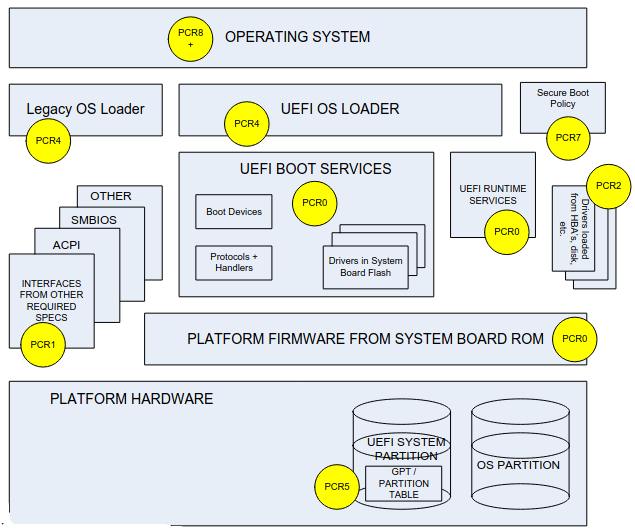
\includegraphics[width=0.5\textwidth]{img/TCG PC Client.png}
  \label{fig:TCG PC Client PCR use}
\end{wrapfigure}

  \item PCR0 is measuring the Platform firmware from system board ROM
    and it is a fixed value given one version of the firmware.
    Typically, in a database there are different values for PCR0
    according to the version of the firmware and the version running
    in a device could be deduced by these values. It also stores the
    UEFI boot services, UEFI runtime services.
  \item PCR1 contains the hash of various extensions of the firmware
    (ACPI, SMBIOS, OTHER).
  \item PCR2 drivers loaded from the disk.
  \item PCR3 is not here. That means it's not used for PC.
  \item PCR4 is the part of the UEFI OS loader and of the Legacy OS
    Loader
  \item PCR5 is for the Platform hardware, for example it is reading
    and computing the hash of the partition table. That is important
    if someone manipulated the hardware.
  \item PCR7 contains the Policy for Secure Boot.
  \item All registers from PCR8 to above are given to the OS to decide
    what will be used for.
\end{itemize}
For all the registers up to PCR7 the values can be predicted. They
will depend on the kind of platform, version of the firmware or
driver. These values are in the golden: if there are wrong values in
those registers the system cannot be trusted.
\begin{table}[H]
  \centering
  \begin{tabular}{|p{0.1\textwidth}|p{0.9\textwidth}|}
    \hline
    \textbf{PCR Index} & \textbf{PCR Usage} \\ \hline
    0 & SRTM, BIOS, Host Platform Extensions, Embedded Option ROMs and PI Drivers \\ \hline
    1 & Host Platform Configuration \\ \hline
    2 & UEFI driver and application Code \\ \hline
    3 & UEFI driver and application Configuration and Data \\ \hline
    4 & UEFI Boot Manager Code (usually the MBR) and Boot Attempts \\ \hline
    5 & Boot Manager Code Configuration and Data (for use by the Boot Manager Code) and GPT/Partition Table \\ \hline
    6 & Host Platform Manufacturer Specific \\ \hline
    7 & Secure Boot Policy \\ \hline
    8-15 & Defined for use by the Static OS \\ \hline
    16 & Debug \\ \hline
    23 & Application Support \\ \hline
  \end{tabular}
  \caption{PCR Index and Usage}
  \label{table:pcr_usage}
\end{table}

